% !TEX program = xelatex
% =============================================================================
%  全国大学生数学建模竞赛（CUMCM）LaTeX 模板
%  字体依赖（正文宋体 / 标题黑体 / 强调楷体）：SimSun / SimHei / KaiTi
%  编译方式：xelatex main.tex（需运行两遍以生成目录）
% =============================================================================
\documentclass[fontset=windows, 12pt, a4paper]{ctexart}

\usepackage[a4paper, top=2.5cm, bottom=2.5cm, left=2.5cm, right=2.5cm]{geometry}
\usepackage{amsmath,amssymb}
\usepackage{graphicx}
\usepackage{float}
\usepackage{multirow}
\usepackage{longtable}
\usepackage[hidelinks]{hyperref}
\graphicspath{{../figures/}}

\IfFontExistsTF{Times New Roman}{\setmainfont{Times New Roman}}{}
\IfFontExistsTF{Consolas}{\setmonofont{Consolas}}{}

\linespread{1.43}
\setlength{\parindent}{2em}

\ctexset{
  section/number       = \chinese{section},
  subsection/number    = \arabic{section}.\arabic{subsection},
  subsubsection/number = \arabic{section}.\arabic{subsection}.\arabic{subsubsection},
}

\usepackage{titlesec}
\titleformat{\section}
  {\centering\fontsize{17.3pt}{20.8pt}\heiti\bfseries}
  {\chinese{section}、}{1em}{}
\titleformat{\subsection}
  {\fontsize{14.45pt}{17.4pt}\heiti\bfseries}
  {\arabic{section}.\arabic{subsection}}{1em}{}
\titleformat{\subsubsection}
  {\fontsize{12.05pt}{14.5pt}\heiti\bfseries}
  {\arabic{section}.\arabic{subsection}.\arabic{subsubsection}}{1em}{}
\titlespacing{\section}       {0pt}{1.25em}{0.82em}
\titlespacing{\subsection}    {0pt}{1.15em}{0.55em}
\titlespacing{\subsubsection} {0pt}{1.15em}{0.55em}

\usepackage{tocloft}
\renewcommand{\cftsecfont}{\heiti\bfseries}
\renewcommand{\cftsecpagefont}{\heiti\bfseries}
\renewcommand{\cftsecleader}{\cftdotfill{\cftdotsep}}
\renewcommand{\cftsubsecleader}{\cftdotfill{\cftdotsep}}
\renewcommand{\cftsubsubsecleader}{\cftdotfill{\cftdotsep}}

\usepackage{booktabs}
\usepackage{array}
\usepackage{xcolor}
\usepackage{listings}
\lstset{
  basicstyle=\ttfamily\scriptsize,
  backgroundcolor=\color{black!3},
  frame=single,
  framesep=5pt,
  rulecolor=\color{black!30},
  framerule=0.7pt,
  breaklines=true,
  showstringspaces=false,
  columns=flexible,
  keepspaces=true,
}

\pagestyle{plain}

\newcommand{\papertitle}[1]{%
  \thispagestyle{empty}%
  \begin{center}
    {\fontsize{17.3pt}{22pt}\bfseries #1}
  \end{center}
  \vspace{1em}
}
\newcommand{\abstractcn}[2]{%
  \thispagestyle{empty}%
  \begin{center}{\fontsize{14pt}{17pt}\bfseries 摘要}\end{center}
  #1\par
  \vspace{1em}
  {\heiti\bfseries 关键字：}#2\par
  \newpage
}
\makeatletter
\newcommand{\tocpage}{%
  \setcounter{page}{1}%
  \begin{center}
    {\fontsize{17.3pt}{20.8pt}\heiti\bfseries 目录}
  \end{center}
  \vspace{0.5em}
  \@starttoc{toc}%
  \newpage
}
\makeatother
\newcommand{\referencescn}{%
  \addcontentsline{toc}{section}{参考文献}%
  % 参考文献。main.tex 的 \referencescn 已自动生成“参考文献”一级标题，
% 本文件不要再写一级标题。

\begin{thebibliography}{99}
\bibitem{boyd2004} Boyd S, Vandenberghe L. Convex Optimization[M]. Cambridge: Cambridge University Press, 2004.
\bibitem{hyndman2021} Hyndman R J, Athanasopoulos G. Forecasting: Principles and Practice[M]. 3rd ed. Melbourne: OTexts, 2021.
\bibitem{virtanen2020} Virtanen P, Gommers R, Oliphant T E, et al. SciPy 1.0: Fundamental Algorithms for Scientific Computing in Python[J]. Nature Methods, 2020, 17: 261--272.
\bibitem{morales2014} Morales J M, Conejo A J, Madsen H, Pinson P, Zugno M. Integrating Renewables in Electricity Markets: Operational Problems[M]. New York: Springer, 2014.
\bibitem{porteus2002} Porteus E L. Foundations of Stochastic Inventory Theory[M]. Stanford: Stanford University Press, 2002.
\bibitem{zipkin2000} Zipkin P H. Foundations of Inventory Management[M]. New York: McGraw-Hill, 2000.
\bibitem{huang2021} 黄元生, 张利君. 考虑需求响应与储能参与的微网日前经济调度[J]. 电力系统保护与控制, 2021, 49(6): 88--96.
\bibitem{wang2020} 王成山, 武震, 李鹏. 微电网关键技术研究[J]. 电工技术学报, 2020, 35(12): 2509--2520.
\end{thebibliography}
%
}
\newcommand{\appendixcn}{%
  \section*{附录 A\quad 核心代码}%
  \addcontentsline{toc}{section}{附录 A\quad 核心代码}%
  % 附录 A：核心代码。只列模型最关键的三段：线性规划、安全裕度与滚动修正。
% 完整工程见 code/ 目录。

\subsection*{A.1\quad 统一线性规划求解器（\texttt{code/core.py}）}

\begin{lstlisting}[language=Python]
def solve_plan(load, pv, price, soc_start, soc_end=None,
               soc_end_value=None, base_purchase=None):
    """求解一组日前计划。
    load / pv : 区间电量预测 kWh，长度 n
    price     : 区间电价 元/kWh
    soc_start : 决策时刻的储电量 kWh
    soc_end   : 若给定，强制收尾储电量等于该值（问题1、日循环口径）
    base_purchase : 若非 None，表示滚动调整，按 0.5*p*|x - base_purchase| 结算偏差
    """
    n = len(load)
    if soc_end_value is None:
        soc_end_value = float(np.mean(price))
    adjusted = base_purchase is not None
    x, c, d, s, w = 0, n, 2 * n, 3 * n, 4 * n
    up, down = 5 * n, 6 * n
    nvar = 5 * n + (2 * n if adjusted else 0)

    # 目标：购电费 + 偏差违约费 + 终端电量残值
    obj = np.zeros(nvar)
    obj[x:x + n] = price
    if adjusted:
        obj[up:up + n] = 0.5 * price      # 增购按 1.5 倍、减购按 0.5 倍，
        obj[down:down + n] = 0.5 * price  # 合并后就是 0.5*p*|x - base|
    obj[c:c + n] = 1e-8                   # 微量惩罚，避免同价时解不唯一
    obj[d:d + n] = 1e-8
    obj[w:w + n] = 1e-9
    obj[s + n - 1] = -soc_end_value

    # 等式约束：功率平衡 + SOC 递推 (+ 调整量定义 + 收尾电量)
    rows = 2 * n + (n if adjusted else 0) + (1 if soc_end is not None else 0)
    A = lil_matrix((rows, nvar)); b = np.zeros(rows)
    for t in range(n):
        A[t, x + t] = 1.0; A[t, d + t] = 1.0
        A[t, c + t] = -1.0; A[t, w + t] = -1.0
        b[t] = load[t] - pv[t]
        A[n + t, s + t] = 1.0
        A[n + t, c + t] = -ETA_CHARGE          # 充电效率 0.9
        A[n + t, d + t] = 1.0 / ETA_DISCHARGE  # 放电效率 1.0
        if t == 0: b[n + t] = soc_start
        else:      A[n + t, s + t - 1] = -1.0
    if adjusted:
        for t in range(n):
            A[2 * n + t, x + t] = 1.0
            A[2 * n + t, up + t] = -1.0
            A[2 * n + t, down + t] = 1.0
            b[2 * n + t] = base_purchase[t]
    if soc_end is not None:
        A[rows - 1, s + n - 1] = 1.0; b[rows - 1] = soc_end

    bounds = ([(0.0, None)] * n            # 购电量非负（不允许售电）
              + [(0.0, FLOW_MAX)] * n      # 充电功率上限 5000/6 kWh
              + [(0.0, FLOW_MAX)] * n      # 放电功率上限 5000/6 kWh
              + [(SOC_MIN, SOC_MAX)] * n   # 储电量 1200 ~ 10800 kWh
              + [(0.0, None)] * n)         # 弃光量
    if adjusted:
        bounds += [(0.0, None)] * (2 * n)

    res = linprog(obj, A_eq=A.tocsr(), b_eq=b, bounds=bounds, method="highs")
    if not res.success:
        raise RuntimeError(f"线性规划求解失败：{res.message}")
    v = res.x
    return Dispatch(purchase=v[x:x + n].copy(), charge=v[c:c + n].copy(),
                    discharge=v[d:d + n].copy(), soc=v[s:s + n].copy(),
                    curtail=v[w:w + n].copy(), cost=float(res.fun))
\end{lstlisting}

\subsection*{A.2\quad 因果预测与报童安全裕度（\texttt{code/forecast.py}）}

\begin{lstlisting}[language=Python]
def history_mean_forecast(series, day, window=7):
    """第 day 天之前 window 天的平均值；第 0 天没有历史，退化为当天实际。"""
    lo = max(0, day - window)
    if lo == day:
        return series[day].copy()
    return series[lo:day].mean(axis=0)


def safety_margin(ins, day, start=0, release_hour=None, window=28, quantile=0.8):
    """区间 [start, 144) 上的安全裕度：历史预测误差的 0.8 分位点。

    紧急购电价是正常价的 5 倍。多买 1 kWh 的边际成本是 p（买多了只能弃掉），
    少买 1 kWh 的边际成本是 5p*P(缺电)，两者相等时 P(缺电) = 1/5，
    所以最优裕度恰好是误差分布的 0.8 分位点——标准的报童模型结论。
    """
    lo = max(1, day - window)
    if lo >= day:
        return np.zeros(len(ins.load[day]) - start)
    errors = np.array([forecast_error(ins, d, start, release_hour)
                       for d in range(lo, day)])
    return np.maximum(np.quantile(errors, quantile, axis=0), 0.0)


def forecast_error(ins, day, start=0, release_hour=None):
    """逐区间预测误差 e = 负载误差 - 光伏误差；e>0 表示当天会缺电。"""
    fc_load = history_mean_forecast(ins.load, day)[start:]
    fc_pv = (history_mean_forecast(ins.pv, day)[start:] if release_hour is None
             else pv_forecast_after(ins, day, release_hour))
    return (ins.load[day, start:] - fc_load) - (ins.pv[day, start:] - fc_pv)
\end{lstlisting}

\subsection*{A.3\quad 问题三的滚动修正主循环（\texttt{code/p3.py}）}

\begin{lstlisting}[language=Python]
def run_problem3(ins, releases=RELEASE_HOURS):
    """滚动求解问题3。releases 可以只给 (0,)，用来做“不滚动”的对照。"""
    records = []
    soc = SOC_INIT
    for day in range(len(ins.dates)):
        fc_load = history_mean_forecast(ins.load, day)
        price = ins.a1_price

        # ---- 0:00 初始计划 ----
        base = solve_plan(fc_load, pv_forecast_after(ins, day, 0), price,
                          soc_start=soc, soc_end=soc)
        base_purchase = base.purchase + safety_margin(ins, day, 0, 0)
        purchase = base_purchase.copy()
        charge, discharge = base.charge.copy(), base.discharge.copy()

        # ---- 后续预报时刻的滚动调整：只重排该时刻之后的区间 ----
        for hour in releases[1:]:
            start = hour * 6
            soc_now = roll_soc(charge[:start], discharge[:start], soc)[-1]
            sub = solve_plan(fc_load[start:], pv_forecast_after(ins, day, hour),
                             price[start:], soc_start=soc_now, soc_end=soc,
                             base_purchase=base_purchase[start:])
            purchase[start:] = sub.purchase + safety_margin(ins, day, start, hour)
            charge[start:] = sub.charge
            discharge[start:] = sub.discharge

        soc_track = roll_soc(charge, discharge, soc)
        real = settle(ins.load[day], ins.pv[day], price, purchase, charge, discharge,
                      purchase_plan=base_purchase)
        records.append(dict(day=day, base=base, base_purchase=base_purchase,
                            purchase=purchase, charge=charge, discharge=discharge,
                            soc_start=soc, soc_end=soc_track[-1],
                            soc_track=soc_track, real=real))
        soc = soc_track[-1]
    return records
\end{lstlisting}

\subsection*{A.4\quad 附件 3 的时间对齐（\texttt{code/forecast.py}）}

\begin{lstlisting}[language=Python]
def pv_forecast_after(ins, day, release_hour):
    """第 release_hour 时发布的预报，对应 release_hour 之后各 10 分钟区间的预测电量。

    附件3 的“预报h小时”指发布时刻起第 h 个小时，即区间 (T+h-1, T+h]，
    所以发布时刻 6:00 的“预报1小时”正好是当天 6:00-7:00，即第 36 个十分钟区间。
    一天只关心到 24:00，因此取前 (24 - release_hour) 个小时即可。
    """
    index = RELEASE_HOURS.index(release_hour)
    hours = ins.pv_fc[day, index][: 24 - release_hour]
    return np.repeat(hours, 6)
\end{lstlisting}
%
}
% 三线表：\threelinetable{标题}{列定义}{表头}{内容}。用 minipage 包住，避免标题与表体被分页拆开
\newcommand{\threelinetable}[4]{%
  \begin{center}
  \begin{minipage}{\linewidth}
    \centering
    {\fontsize{10.5pt}{12.6pt}\heiti\bfseries #1}\par
    \vspace{0.5em}
    \begin{tabular}{#2}
      \toprule
      #3 \\
      \midrule
      #4 \\
      \bottomrule
    \end{tabular}
  \end{minipage}
  \end{center}
}

\begin{document}

\papertitle{基于报童安全裕度与滚动修正的微网购电与储能调度模型}

\abstractcn{%
本文针对含光伏与储能的非孤岛式微网，在 10 分钟粒度上建立了“确定性线性规划 + 报童安全裕度 + 滚动修正”的统一调控框架，并用 2025 年 2 月至 12 月的全年数据完成因果回测。

针对\textbf{问题一}，建立以全天购电费用最小为目标的确定性线性规划，约束包括功率平衡、储电量上下限、充放电功率上限以及 0:00 与 24:00 储电量相等（均为 $6000\,\mathrm{kWh}$）。求解得到全天购电量 $57580.98\,\mathrm{kWh}$、购电费 $33416.53$ 元；储能于 0:00--4:00 低价时段充电 $4500.00\,\mathrm{kWh}$，16:00--20:00 高价时段放电 $6740.13\,\mathrm{kWh}$ 顶负荷，白天光伏富余时段补充充电，全天无弃光。

针对\textbf{问题二}，以决策时刻之前 7 天的历史均值作为负载与光伏的日前预测，并利用紧急购电价为正常电价 5 倍这一非对称代价，把计划购电量加上预测误差分布的 $q$ 分位点作为安全裕度。由报童模型，边际成本相等给出 $P(e_t>y_t)=1/5$，即最优分位点 $q=0.8$；实测全年费用曲线的最低点恰在 $q=0.80$，比不加裕度节省 $693$ 万元（$29\%$）。2025 年 2 月 1 日至 12 月 31 日计划购电 $2436.83$ 万 $\mathrm{kWh}$、紧急购电 $34.38$ 万 $\mathrm{kWh}$（占负载 $0.929\%$），总购电费用 $1702.64$ 万元。

针对\textbf{问题三}，将附件 3 的整点光伏预报按 $(\text{发布时刻}+h-1,\ \text{发布时刻}+h]$ 展开到 10 分钟区间，在 0:00 制定初始计划，并在 6:00、12:00、18:00 只重排尚未执行的时段。推导并采用对称的偏差结算式 $\sum p_t x_t^{\text{adj}}+0.5\sum p_t|x_t^{\text{adj}}-x_t^{\text{plan}}|$，它同时覆盖“增购按 1.5 倍、减购按 0.5 倍”两条规则。滚动方案总费用 $1760.56$ 万元，比只用 0:00 预报的 $1780.62$ 万元\textbf{净省 $20.06$ 万元}，紧急购电由 $36.67$ 万降至 $26.82$ 万 $\mathrm{kWh}$，结论是值得引入。

针对\textbf{问题四}，以实时电价的 7 日均值制定计划、按实际电价结算。对应问题二的方案总费用 $1734.13$ 万元，对应问题三的方案 $1782.78$ 万元；波动电价相比固定电价多支出约 $31.5$ 万元，全部来自价格预测误差。

全文所有方案的能量平衡等式最大残差不超过 $4.6\times10^{-12}\,\mathrm{kWh}$，储电量与充放电功率边界违反不超过 $3.6\times10^{-12}$，且每一天的日前决策都经过“不使用当日及以后信息”的断言校验。%
}{%
微网调度 \quad 储能优化 \quad 报童模型 \quad 滚动修正 \quad 线性规划%
}

\tocpage

\section{问题重述}

\subsection{问题背景}

微网是为解决光伏发电等分布式能源本地消纳、减少并网问题而发展起来的小型发用电系统。出于经济考虑，非孤岛式微网可以在外网电价较低或分布式能源有剩余的时间段为储能设备充电，并在外网电价较高的时间段释放电能。调控的目标是利用小区负载、光伏发电量与储能当前储电量等数据，尽可能精准地给出微网购电量与储能充放电量，使微网既满足小区负载，又尽可能节省购电费用。

\subsection{储能设备参数}

储能最大容量 $12000\,\mathrm{kWh}$，允许储电量范围 $1200\sim10800\,\mathrm{kWh}$，最大充放电功率 $5000\,\mathrm{kW}$，充放电效率 $90\%$（充入 $1\,\mathrm{kWh}$ 有 $0.9\,\mathrm{kWh}$ 进入电池，放出 $1\,\mathrm{kWh}$ 电池减少 $1\,\mathrm{kWh}$）。2025 年 1 月 1 日 0:00 的电量为 $6000\,\mathrm{kWh}$。调度间隔为 10 分钟，每天 144 个区间。

\subsection{需要解决的问题}

\textbf{问题一}：每天的电价和小区负载相同，并给出一天的光伏发电功率预测，要求微网提供的电能不低于小区负载，且储能设备在 0:00 与 24:00 的储电量相同。建立数学模型，给出指定 10 分钟区间的购电量、全天购电量与购电费、六个 4 小时时段的充放电量及首尾储电量。

\textbf{问题二}：每天电价相同，但小区负载和光伏发电功率随日期和时间变化。若正常购电、光伏和储能仍不能满足负载，需按交易时刻电价的 5 倍紧急购电；除此以外其他购电费用按计划购电量计算。每天 0:00 制定当天计划，对 2025 年 2 月 1 日至 12 月 31 日给出计划购电量、充放电量、连续紧急购电区间及电量。

\textbf{问题三}：每天 0:00、6:00、12:00、18:00 可获得未来 24 小时整点的光伏发电功率预报。0:00 的预报用于制定初始计划，后续预报可用于调整尚未执行的购电计划。计划购电量高于调整购电量的部分按交易时刻电价的 $50\%$ 承担违约费用；调整购电量高于计划购电量的部分按交易时刻电价的 $1.5$ 倍购入。总费用包括计划购电费用、紧急购电费用和调整相关费用。要求给出完整的初始计划、调整计划、最终储能调度与紧急购电，并分析是否需要引入其他时刻的预报。

\textbf{问题四}：外网电价按日期和 10 分钟区间实时波动，使用附件 4 的数据重新计算问题二与问题三，并给出相应成本与策略的比较。

\section{问题分析}

\subsection{数据口径的三处关键确认}

\textbf{功率与电量的换算。}附件给出的电价单位是元/$\mathrm{kWh}$，负载与光伏单位是 $\mathrm{kW}$，而结果表要求填写 $\mathrm{kWh}$。10 分钟区间内功率近似恒定，故区间电量等于功率乘以 $1/6\,\mathrm{h}$。储能 $5000\,\mathrm{kW}$ 的功率上限对应每区间 $5000/6\approx833.333\,\mathrm{kWh}$ 的能量上限。

\textbf{附件 3 的时间对齐。}附件 3 每行是一次预报，“预报 $h$ 小时”指发布时刻起第 $h$ 个小时，即区间 $(\text{发布时刻}+h-1,\ \text{发布时刻}+h]$。以 2025-06-21 为例，0:00 发布的“预报 6 小时”为 $2533\,\mathrm{kWh}$，而当天 5:00--6:00 的实际光伏为 $1905\,\mathrm{kWh}$；“预报 6 小时”若解释成 6:00--7:00 则与实际 $3405\,\mathrm{kWh}$ 相差更大。逐小时相关分析也支持该对齐：按此对齐，4:00--17:00 各小时的预报与实际相关系数均在 $0.84$ 以上。使用时在该小时的 6 个十分钟区间内取常值。

\textbf{附件 5 模板的表头错位。}模板“计划购电量”工作表的第一行标签是 \texttt{0:10-0:20}，最后一行是 \texttt{0:00+1-0:10+1}，比当天实际的 144 个区间整体错开一格（当天的第一个区间应为 0:00--0:10）。由于题目要求不得改动模板结构，本文按行号映射：第 2 行填写第 0 个区间，第 145 行填写第 143 个区间，并在结果报告中披露该风险。附件 1、附件 2、附件 4 的“时间”列同样是区间结束时刻（0:10 至 0:00+1），与本映射自洽。

\subsection{各问的思路}

\textbf{问题一}是确定性优化：电价、负载、光伏预测全部给定，储能首尾电量相等。它本质是一个带储能递推约束的线性规划\cite{boyd2004}，可以用单纯形法一次求解。

\textbf{问题二}引入两类不确定性。其一是负载与光伏的真实值偏离预测值；其二是紧急购电的价格高达正常电价的 5 倍。题面没有给出问题二的日前预测数据，因此必须自行构造一个只使用决策时刻以前信息的因果预测\cite{hyndman2021}。取此前 7 天的历史均值作为预测，同时必须处理 $5$ 倍非对称代价：买多了只能弃掉（损失 $1$ 倍电价），买少了要按 $5$ 倍价补购，所以最优计划不应等于预测值，而应在其上叠加一个安全裕度。

\textbf{问题三}提供了更准的光伏信息。要求把附件 3 的整点预报展开到 10 分钟粒度，在四个预报时刻滚动重排尚未执行的时段，并按“增购 1.5 倍、减购 0.5 倍”结算偏差。问题的落脚点是：这些后续预报究竟值多少钱。

\textbf{问题四}把电价也变成随机量。电价同样只能在 0:00 之前观测，因此计划用历史均值价制定、按实际价结算，两者的差额就是价格预测误差的代价。

\subsection{贯穿四问的一个恒等式}

在“储能严格按计划充放电”的执行口径下，把计划的功率平衡式
$x_t+PV_t^{\text{fc}}+d_t-c_t-w_t=L_t^{\text{fc}}$
代入执行缺额 $\text{gap}_t=L_t+c_t-PV_t-d_t-x_t$，得到
\begin{equation}
\text{gap}_t=e_t-w_t,\qquad
e_t=\bigl(L_t-L_t^{\text{fc}}\bigr)-\bigl(PV_t-PV_t^{\text{fc}}\bigr),
\label{eq:identity}
\end{equation}
其中 $e_t$ 是净负荷的预测误差。\textbf{缺额与储能的充放电决策无关}，只由预测误差和计划内弃光量决定。这个恒等式有两个直接推论：第一，问题二中紧急购电只能靠“多买”（即 $w_t>0$）来压缩，不能靠储能调度；第二，问题三压缩的是同一个 $e_t$，因此预报精度的提升可以直接换算成紧急购电费用的下降。全文的问题二至问题四都围绕这条主线展开。

\section{模型假设}

\begin{enumerate}
  \item \textbf{功率分段恒定。}每个 10 分钟区间内电价、负载与光伏功率视为常数，区间电量等于功率乘以 $1/6\,\mathrm{h}$。
  \item \textbf{充放电效率全记在充电侧。}按附录 1 的“充放电效率 $90\%$”，本文取充入 $1\,\mathrm{kWh}$ 有 $0.9\,\mathrm{kWh}$ 进入电池、放出 $1\,\mathrm{kWh}$ 电池减少 $1\,\mathrm{kWh}$，完整充放一次为 $0.9$。
  \item \textbf{不允许向外网售电。}光伏富余时只能给储能充电或弃光，因此计划中显式设置弃光变量 $w_t\ge0$，且购电量 $x_t\ge0$。
  \item \textbf{储能在日前计划内严格按曲线充放电。}执行阶段实际负载与光伏一旦偏离预测，差额全部由紧急购电（不足）或弃光（有余）吸收，储能不临时改变充放电量。这既是题面“制定计划购电策略”的自然含义，也是式~\eqref{eq:identity} 成立的前提。
  \item \textbf{日前决策严格因果。}第 $d$ 天 0:00 的计划只允许使用第 $d-1$ 天及更早的历史数据；问题三中 $6{:}00$、$12{:}00$、$18{:}00$ 的调整只允许使用该时刻已发布的预报。任何时刻都不得读取当天未来的实际值。
  \item \textbf{储能日循环运行。}问题一中储能 0:00 与 24:00 的储电量相等且均为 $6000\,\mathrm{kWh}$；问题二至四把该口径推广为每天计划结束时回到当天起始电量。由于电价日型固定，跨日套利的空间很小，该假设的代价在灵敏度分析中量化。
  \item \textbf{计划内弃光等价于预留裕度。}计划中出现的弃光量 $w_t>0$ 表示“按预测多买、多买的电在预测兑现时弃掉”，它是应对预测误差的保险，而非设备故障。
\end{enumerate}

\section{符号说明}

\begin{center}
{\fontsize{10.5pt}{12.6pt}\heiti\bfseries 表 1\quad 主要符号}\par
\vspace{0.5em}
\begin{tabular}{clc}
\toprule
符号 & 含义 & 单位 \\
\midrule
$t$ & 区间下标，$t=0,1,\dots,143$，第 $t$ 段为 $t/6$ 时至 $(t+1)/6$ 时 & --- \\
$N$ & 每天区间数，$N=144$ & --- \\
$\Delta t$ & 区间长度，$\Delta t=1/6$ & h \\
$L_t,\ PV_t$ & 小区负载、光伏发电的实际区间电量 & kWh \\
$L_t^{\mathrm{fc}},\ PV_t^{\mathrm{fc}}$ & 负载、光伏的日前预测区间电量 & kWh \\
$p_t$ & 区间电价 & 元/kWh \\
$x_t$ & 计划购电量 & kWh \\
$\tilde x_t$ & 调整后的购电量（问题三、四） & kWh \\
$c_t,\ d_t$ & 储能充电量、放电量 & kWh \\
$s_t$ & 第 $t$ 段结束时的储电量 & kWh \\
$w_t$ & 计划内弃光量（等于安全裕度） & kWh \\
$e_t$ & 净负荷预测误差，见式~\eqref{eq:identity} & kWh \\
$y_t$ & 安全裕度，取误差分布的 $q$ 分位点 & kWh \\
$q$ & 安全裕度分位点，$q=0.8$ & --- \\
$E_t$ & 紧急购电量 & kWh \\
$\eta_c,\ \eta_d$ & 充电效率、放电效率，$\eta_c=0.9$，$\eta_d=1$ & --- \\
$S^{\min},S^{\max}$ & 储电量上下限，$1200$、$10800$ & kWh \\
$P^{\max}$ & 最大充放电功率，$5000$ & kW \\
$r$ & 预报发布时刻，$r\in\{0,6,12,18\}$ & 时 \\
\bottomrule
\end{tabular}
\end{center}

\section{问题一：确定性线性规划模型}

\subsection{模型建立}

问题一中电价、负载与光伏预测全天已知，储能首尾电量相等，是一个确定性优化问题。以全天购电费用最小为目标，决策变量为 144 个区间的购电量 $x_t$、充电量 $c_t$、放电量 $d_t$、储电量 $s_t$ 与弃光量 $w_t$。

\begin{equation}
\min_{x,c,d,s,w}\quad \sum_{t=0}^{N-1} p_t x_t
\label{eq:p1obj}
\end{equation}

约束条件如下。

\textbf{功率平衡}（等式，不允许售电）：
\begin{equation}
x_t+PV_t+d_t-c_t-w_t=L_t,\qquad t=0,\dots,N-1 .
\label{eq:p1balance}
\end{equation}

\textbf{储能递推与容量}：
\begin{equation}
s_t=s_{t-1}+\eta_c c_t-\frac{d_t}{\eta_d},\quad
s_{-1}=s_{N-1}=S_0=6000,\quad
S^{\min}\le s_t\le S^{\max}.
\label{eq:p1soc}
\end{equation}

\textbf{充放电功率与购电边界}：
\begin{equation}
0\le c_t\le P^{\max}\Delta t,\qquad
0\le d_t\le P^{\max}\Delta t,\qquad
x_t\ge0,\qquad w_t\ge0 .
\label{eq:p1bounds}
\end{equation}

式~\eqref{eq:p1balance}--\eqref{eq:p1bounds} 全部是线性等式或线性不等式，式~\eqref{eq:p1obj} 是线性目标，因此这是一个标准线性规划\cite{boyd2004}，采用 HiGHS 单纯形法求解\cite{virtanen2020}。变量共 $5\times144=720$ 个，等式约束 $2\times144+1=289$ 条。

\subsection{求解结果}

求解得到全天购电量 $57580.98\,\mathrm{kWh}$、全天购电费 $33416.53$ 元，储能 0:00 与 24:00 的储电量均为 $6000.00\,\mathrm{kWh}$，全天弃光为 $0$。表 2、表 3 给出论文要求的展示口径。

\threelinetable{表 2\quad 指定时间段购电量与全天合计}{lrlr}
{时间段 & 购电量 / kWh & 时间段 & 购电量 / kWh}
{10:00-10:10 & 0.0000 & 16:00-16:10 & 445.4317 \\
 12:00-12:10 & 480.4124 & 18:00-18:10 & 0.0000 \\
 14:00-14:10 & 0.0000 & 20:00-20:10 & 0.0000 \\
 \multicolumn{3}{l}{全天购电量 / kWh} & 57580.98 \\
 \multicolumn{3}{l}{全天购电费 / 元} & 33416.53}

\threelinetable{表 3\quad 储能设备分时段充放电量与首尾储电量}{lrr}
{时间段 & 充电量 / kWh & 放电量 / kWh}
{0:00-4:00   & 4500.0000 & 0.0000 \\
 4:00-8:00   & 833.3333  & 6956.9814 \\
 8:00-12:00  & 4448.6339 & 1702.9970 \\
 12:00-16:00 & 5274.7881 & 91.1014 \\
 16:00-20:00 & 0.0000    & 6740.1319 \\
 20:00-24:00 & 5333.3333 & 2859.8681 \\
 \multicolumn{2}{l}{0:00 储电量 / kWh} & 6000.00 \\
 \multicolumn{2}{l}{24:00 储电量 / kWh} & 6000.00}

\begin{figure}[H]
  \centering
  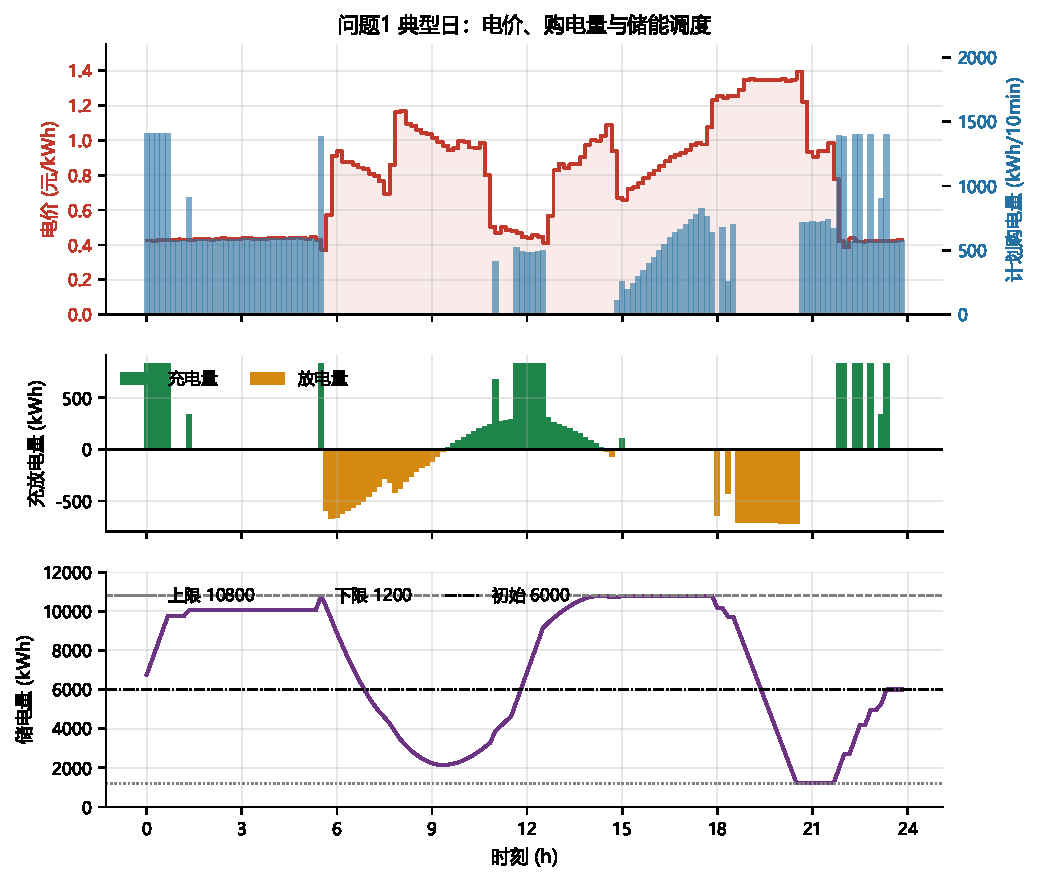
\includegraphics[width=0.94\textwidth]{p1_dispatch.pdf}
  \caption{问题一典型日的电价、计划购电量、储能充放电量与储电量}
  \label{fig:p1}
\end{figure}

图~\ref{fig:p1} 显示调度策略呈现清晰的“低价充、高价放”结构，储电量轨迹可以分为四段。

\textbf{夜间低价充电（0:00--5:30）。}此时电价处于 $0.42\sim0.43$ 元/$\mathrm{kWh}$ 的当日低位，储能以接近上限的功率充电，储电量从 $6000\,\mathrm{kWh}$ 升至 $10050\,\mathrm{kWh}$ 并于 5:30 触及 $10800\,\mathrm{kWh}$ 的上限。

\textbf{早高峰放电（5:30--10:00）。}光伏出力尚小，小区负载在 9:00 附近达到全天最大值 $993.16\,\mathrm{kWh}$/区间（对应 $5959\,\mathrm{kW}$），储能放电顶负荷。储电量从上限回落到 10:00 的 $2279\,\mathrm{kWh}$，其间 5:40--8:00 等 61 个区间购电量降为 $0$。

\textbf{白天光伏富余充电（10:00--16:00）。}全天有 30 个区间光伏出力超过小区负载，富余总量 $6248.0\,\mathrm{kWh}$，全部被储能吸收，没有弃光。储电量从 $2279\,\mathrm{kWh}$ 回升并在 16:00 重新触顶 $10800\,\mathrm{kWh}$，16:00--18:00 维持满电待发。

\textbf{晚高峰放电与回充（18:00--24:00）。}电价进入 $1.3$ 元/$\mathrm{kWh}$ 以上的峰段，储能集中放电，储电量在 20:30 触及 $1200\,\mathrm{kWh}$ 的下限；21:00 之后电价回落，储能再次以低价电补回电量，24:00 精确回到 $6000\,\mathrm{kWh}$。

全天弃光为 $0$，说明储能容量足以吸收全部光伏富余。论文要求的六个展示区间中，10:00--10:10、14:00--14:10、18:00--18:10、20:00--20:10 四个区间购电量均为 $0$，完全由光伏与储能供电。

\section{问题二：带安全裕度的日前计划模型}

\subsection{因果预测}

题目没有给出问题二可用的日前负载与光伏预测，只给了 2025 年全年的实际值。为保证日前决策的因果性，本文取\textbf{此前 7 天的历史均值}作为当天逐区间的预测：
\begin{equation}
L_t^{\mathrm{fc}}=\frac1{7}\sum_{k=1}^{7}L_t^{(d-k)},\qquad
PV_t^{\mathrm{fc}}=\frac1{7}\sum_{k=1}^{7}PV_t^{(d-k)},
\label{eq:fc}
\end{equation}
其中 $L_t^{(d-k)}$ 表示第 $d-k$ 天第 $t$ 个区间的实际值。第 $d$ 天的决策只用到第 $d-1$ 天及更早的数据，满足因果约束。2025 年 1 月为滚动起步的预热月，其结果不计入 2 月至 12 月的交付范围。

在 2025 年 2 月至 12 月上，该预测的精度为：负载平均绝对误差 $130.2\,\mathrm{kWh}$/区间，光伏平均绝对误差 $25.6\,\mathrm{kWh}$/区间。负载误差明显大于光伏误差，因此净负荷误差 $e_t$ 主要由负载主导。

\subsection{计划模型}

第 $d$ 天 0:00 在预测曲线上求解与问题一结构相同的线性规划，但约束改为日循环而非固定首尾电量：
\begin{equation}
s_{-1}=s_{N-1}=s^{(d)}_0,\qquad
S^{\min}\le s_t\le S^{\max},
\label{eq:p2soc}
\end{equation}
其中 $s^{(d)}_0$ 是当天起始的实际储电量。目标函数仍为 $\min\sum_t p_t x_t$。

\subsection{安全裕度：报童模型}

按预测原样购电并不是最优的。由式~\eqref{eq:identity}，执行缺额等于 $e_t-w_t$，而 5 倍的紧急购电价使得“少买”远比“多买”昂贵。设区间 $t$ 上在计划中额外多买 $y_t\ \mathrm{kWh}$（即在计划内多弃光 $y_t$）：

\begin{itemize}
  \item 若实际并不缺电，多买的 $y_t$ 只能弃掉，边际成本为 $p_t$；
  \item 若实际缺电 $e_t>y_t$，多买可以少付 $(e_t-y_t)$ 部分的 5 倍紧急购电费，边际收益为 $5p_t\cdot P(e_t>y_t)$。
\end{itemize}

令两者相等，得到经典报童模型\cite{porteus2002,zipkin2000}的最优条件：
\begin{equation}
p_t=5p_t\,P(e_t>y_t)
\quad\Longrightarrow\quad
P(e_t>y_t)=\frac{1}{5}
\quad\Longrightarrow\quad
y_t=F_{e_t}^{-1}(0.8),
\label{eq:newsvendor}
\end{equation}
即最优安全裕度就是预测误差分布的 $\mathbf{0.8}$ 分位点。实际计算时用此前 28 天同一区间的误差样本估计该分位点，并截断到非负。由于 $y_t$ 只影响购电量与弃光量、不改变储能充放电决策，可以把裕度直接叠加在规划解之上：
\begin{equation}
x_t \leftarrow x_t^{\text{LP}}+y_t,\qquad w_t\leftarrow w_t^{\text{LP}}+y_t .
\label{eq:margin}
\end{equation}

\subsection{求解结果}

表 4 给出不同分位点下的全年费用。实际最优分位点恰为 $q=0.80$，与式~\eqref{eq:newsvendor} 的理论值一致；相比不加裕度，全年节省 $693$ 万元（$29\%$）。

\threelinetable{表 4\quad 安全裕度分位点对问题二全年费用的影响（单位：万元）}{cccc}
{分位点 $q$ & 计划购电费 & 紧急购电费 & 总费用}
{不加裕度 & 1111.3 & 1284.7 & 2396.0 \\
 0.50 & 1382.0 & 446.0 & 1828.0 \\
 0.70 & 1504.9 & 211.4 & 1716.3 \\
 \textbf{0.80} & \textbf{1570.3} & \textbf{132.4} & \textbf{1702.6} \\
 0.90 & 1657.0 & 68.8 & 1725.8}

\begin{figure}[H]
  \centering
  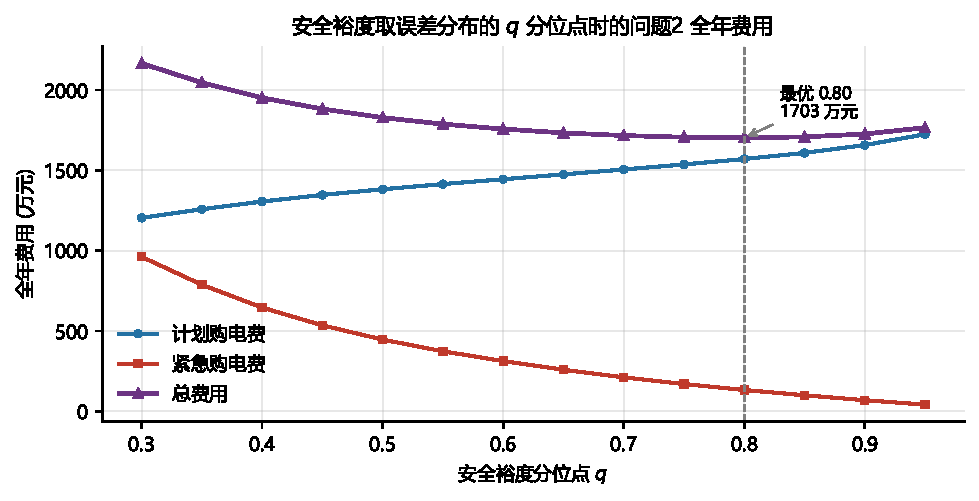
\includegraphics[width=0.72\textwidth]{margin_tradeoff.pdf}
  \caption{安全裕度分位点与全年费用的关系，最低点在 $q=0.80$}
  \label{fig:margin}
\end{figure}

图~\ref{fig:margin} 显示的 U 形曲线正是报童模型的典型形态：分位点越低，紧急购电费越高；分位点越高，计划购电费越高；两者之和在 $q=0.80$ 处最小。

\subsection{全年结果}

2025 年 2 月 1 日至 12 月 31 日共 334 天，结果汇总于表 5。

\threelinetable{表 5\quad 问题二全年结果汇总}{lr}
{指标 & 数值}
{实际负载合计 / kWh & 37008079.49 \\
 计划购电量 / kWh & 24368275.98 \\
 计划购电费 / 元 & 15702558.44 \\
 紧急购电量 / kWh & 343800.18（占负载 $0.929\%$） \\
 紧急购电费 / 元 & 1323841.81 \\
 \textbf{总购电费用 / 元} & \textbf{17026400.25}}

全年 334 天中有 248 天出现过紧急购电，但单次规模有限：逐日紧急购电量的中位数为 $561.19\,\mathrm{kWh}$，最大的一天为 $14118.4\,\mathrm{kWh}$，说明安全裕度已经把大部分预测误差消化在计划内。

\threelinetable{表 6\quad 问题二指定日期的计划购电与紧急购电}{lrrr}
{日期 & 计划购电量 / kWh & 紧急购电量 / kWh & 费用 / 元}
{2025-03-20 & 65644.45 & 1074.66 & 45119.57 \\
 2025-06-21 & 79792.46 & 0.00 & 51753.45 \\
 2025-09-23 & 66247.34 & 1593.46 & 50655.49 \\
 2025-12-21 & 95755.68 & 649.18 & 63386.35}

\begin{figure}[H]
  \centering
  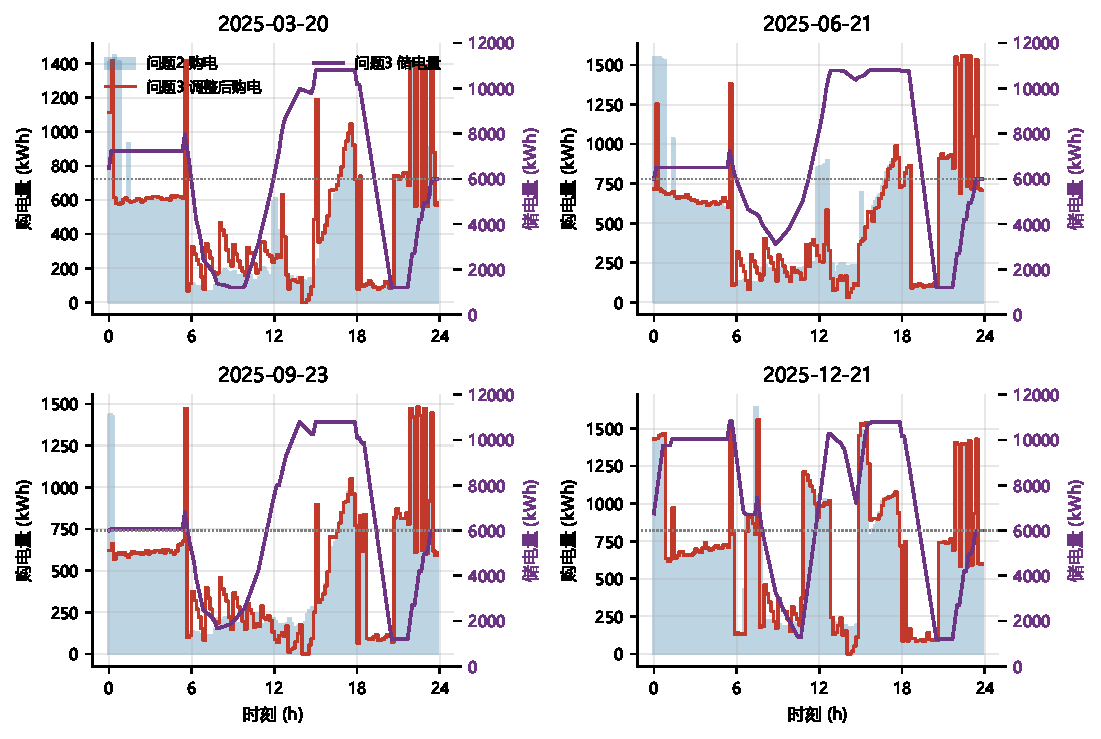
\includegraphics[width=0.95\textwidth]{display_days.pdf}
  \caption{四个指定日期的购电量与储电量，以及问题三调整后的对比}
  \label{fig:days}
\end{figure}

2025 年 6 月 21 日是夏至，光伏出力最强，虽然计划购电量不是全年最大，但当天紧急购电为 0；12 月 21 日负载最重、光伏最弱，计划购电量达 $95755.68\,\mathrm{kWh}$，为四个展示日期中最大，费用也最高。四个日期的紧急购电都集中在夜间与清晨的负载爬升段（如 3 月 20 日的 0:20--0:40、12 月 21 日的 3:30--3:50），因为该时段既没有光伏支撑、又是预测误差最容易被放大的时段。

\section{问题三：光伏预报展开与滚动修正模型}

\subsection{预报的时间对齐}

附件 3 每行是一次预报，“预报 $h$ 小时”指发布时刻起第 $h$ 个小时，即区间 $(\text{发布时刻}+h-1,\ \text{发布时刻}+h]$。例如 6:00 发布的“预报 1 小时”对应当天 6:00--7:00，也就是第 36 个十分钟区间。因此发布时刻 $r$ 的预报展开后正好覆盖区间 $[6r,144)$：
\begin{equation}
PV^{\mathrm{fc}(r)}_{6r+i}=\bigl[\text{附件3 在 }r\text{ 时发布的第 }(i/6+1)\text{ 小时值}\bigr]\,\Delta t,
\qquad i=0,\dots,144-6r-1 .
\label{eq:p3expand}
\end{equation}
即在该小时的 6 个十分钟区间内取常值。

滚动修正在电力市场与微网调度中已有广泛应用\cite{morales2014,wang2020}。

\subsection{滚动修正模型}

\textbf{0:00 初始计划。}用附件 3 的 0:00 预报作为光伏预测、式~\eqref{eq:fc} 的 7 日均值作为负载预测，加上安全裕度式~\eqref{eq:margin}，得到初始计划 $(x^{\text{plan}}_t,c_t,d_t)$。

\textbf{$r\in\{6,12,18\}$ 的调整。}在 $r$ 时刻，区间 $[0,6r)$ 已经执行完毕、不可更改；只对剩余区间 $[6r,144)$ 重新求解线性规划，起点为当前储电量，收尾仍回到当天起始电量。由于引入了更准的预报，剩余时段的光伏预测被替换为 $PV^{\mathrm{fc}(r)}$。

\subsection{偏差结算}

题面给出的两条规则可以合并。设 $\Delta_t=x_t^{\text{adj}}-x_t^{\text{plan}}$。

\textbf{增购}（$\Delta_t>0$）：计划部分按 $p_t$ 计费，超出部分按 $1.5p_t$ 购入，
\begin{equation}
p_tx^{\text{plan}}_t+1.5p_t\Delta_t=p_tx^{\text{adj}}_t+0.5p_t\Delta_t .
\end{equation}

\textbf{减购}（$\Delta_t<0$）：调整后的电量按 $p_t$ 计费，被削减的部分按 $0.5p_t$ 承担违约费，
\begin{equation}
p_tx^{\text{adj}}_t+0.5p_t\bigl(x^{\text{plan}}_t-x^{\text{adj}}_t\bigr)
=p_tx^{\text{adj}}_t+0.5p_t|\Delta_t| .
\end{equation}

两式在各自的分支上完全一致，因此可以统一写成对称的偏差结算式：
\begin{equation}
C_{\text{购电}}=\sum_{t}p_tx^{\text{adj}}_t
+\frac12\sum_t p_t\bigl|x^{\text{adj}}_t-x^{\text{plan}}_t\bigr| .
\label{eq:deviation}
\end{equation}
总费用为 $C=C_{\text{购电}}+5\sum_t p_t E_t$。式~\eqref{eq:deviation} 中的第二项是凸的分段线性函数，用一对非负变量 $u_t,v_t\ge0$ 且 $x^{\text{adj}}_t-u_t+v_t=x^{\text{plan}}_t$ 线性化后仍然是一个标准线性规划。

\subsection{预报精度分析}

表 7 把三种光伏预测放在\textbf{同一时段}上比较平均绝对误差，避免因覆盖窗口不同而产生偏差。

\threelinetable{表 7\quad 三种光伏预测在同一时段上的平均绝对误差（kWh/区间）}{lrrr}
{时段 & 前 7 日均值 & 只用 0:00 预报 & 滚动使用最新预报}
{0:00--6:00   & 0.7  & 6.6   & 6.6 \\
 6:00--12:00  & 52.5 & 114.2 & 98.4 \\
 12:00--18:00 & 48.7 & 123.4 & 92.2 \\
 18:00--24:00 & 0.4  & 3.2   & 3.2 \\
 全天整体     & 25.6 & 61.9  & ---}

\begin{figure}[H]
  \centering
  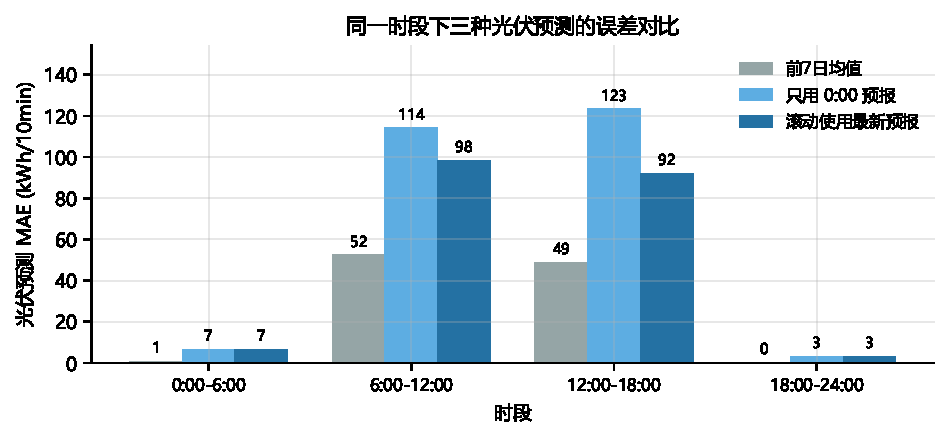
\includegraphics[width=0.86\textwidth]{forecast_accuracy.pdf}
  \caption{同一时段下三种光伏预测的平均绝对误差对比}
  \label{fig:fc}
\end{figure}

两个结论值得注意。第一，\textbf{滚动使用最新预报确实降低了误差}：在 6:00--12:00 段由 $114.2$ 降到 $98.4\ \mathrm{kWh}$，在 12:00--18:00 段由 $123.4$ 降到 $92.2\ \mathrm{kWh}$，降幅分别为 $13.8\%$ 和 $25.3\%$。第二，\textbf{附件 3 的预报本身并不比“前 7 天的实际均值”更准}——全天整体误差 $61.9$ 对 $25.6$，几乎是后者的 2.4 倍。这解释了为什么问题三的总费用高于问题二（同样的安全裕度机制下，预报误差更大）。这也说明，如果允许同时使用两路信息，把附件 3 的预报与历史均值做加权融合还有进一步降本的空间。

\subsection{滚动修正的结果与结论}

\threelinetable{表 8\quad 问题三全年结果对比（2025-02-01 至 2025-12-31）}{lrr}
{指标 & 引入 6/12/18 点预报 & 只用 0:00 预报}
{0:00 计划购电量 / kWh & 25012959.00 & 25012959.00 \\
 调整后购电量 / kWh & 24611319.48 & 25012959.00 \\
 购电费 / 元 & 16130122.56 & 16416828.97 \\
 偏差违约费 / 元 & 454289.21 & 0.00 \\
 紧急购电量 / kWh & 268200.65 & 366664.04 \\
 紧急购电费 / 元 & 1021169.31 & 1389336.28 \\
 \textbf{总购电费用 / 元} & \textbf{17605581.08} & \textbf{17806165.24}}

\textbf{结论：值得引入后续预报。}滚动方案比只用 0:00 预报的方案净省
$17806165.24-17605581.08=\mathbf{200584.16}$ 元/年。分解来看，紧急购电费下降 $36.8$ 万元，而偏差违约费只有 $45.4$ 万元、调整后购电费本身又下降了 $28.7$ 万元，三者相抵后仍净赚 $20.06$ 万元。

另一个值得注意的现象是\textbf{调整方向以减购为主}：调整后购电量 $24611319.48\,\mathrm{kWh}$ 小于 0:00 计划的 $25012959.00\,\mathrm{kWh}$。这说明 0:00 计划在安全裕度的作用下偏保守，后续预报主要起“纠正过度保守”的作用——在确认当天不会缺电之后，把多余的保险退掉（代价是 $0.5$ 倍的违约费）。

\threelinetable{表 9\quad 问题三指定日期的结果}{lrrr}
{日期 & 0:00 计划 / kWh & 调整后 / kWh & 紧急购电 / kWh}
{2025-03-20 & 68068.16 & 66797.62 & 1976.85 \\
 2025-06-21 & 73080.10 & 73578.04 & 0.00 \\
 2025-09-23 & 70044.31 & 66709.12 & 1160.65 \\
 2025-12-21 & 96561.06 & 94489.77 & 1461.53}

四天对应的总费用分别为 $51528.93$、$49997.26$、$50931.20$、$66322.47$ 元。与问题二同期相比，3 月 20 日费用上升（$45119.57\to51528.93$ 元），但 12 月 21 日的紧急购电由 $649.18$ 升到 $1461.53\,\mathrm{kWh}$ 而购电费下降，最终总费用由 $63386.35$ 元升到 $66322.47$ 元——同样是附件 3 预报精度不如历史均值所致。

\section{问题四：波动电价下的重算}

\subsection{价格信息的因果边界}

附件 4 给出的是 2025 年全年的实时电价。与负载和光伏一样，0:00 制定当天计划时无法预知当天的实际电价，因此计划必须建立在价格预测之上，而结算按实际电价进行，这正是电力市场实时结算的典型结构\cite{morales2014,huang2021}。本文沿用与前两问一致的口径，取\textbf{此前 7 天同一时段的平均电价}作为预测：
\begin{equation}
p_t^{\mathrm{fc}}=\frac1{7}\sum_{k=1}^{7}p_t^{(d-k)} .
\label{eq:pricefc}
\end{equation}

价格数据的统计特征是：附件 4 的逐日电价与附件 1 的固定日型高度相关（相关系数均值 $0.971$、中位数 $0.976$），全天均值 $0.7575$ 元/$\mathrm{kWh}$、标准差 $0.3360$ 元/$\mathrm{kWh}$，取值范围 $0.0076\sim1.7936$ 元/$\mathrm{kWh}$。式~\eqref{eq:pricefc} 的预测平均绝对误差为 $0.0827$ 元/$\mathrm{kWh}$，且几乎无系统性偏差（均值偏差 $-0.0003$）。

\subsection{模型}

\textbf{问题 4-2}（对应问题二）：0:00 用 $p^{\mathrm{fc}}$ 求解式~\eqref{eq:p2soc} 的计划并叠加安全裕度式~\eqref{eq:margin}，执行时储能严格按计划充放电，紧急购电按实际电价的 5 倍结算：
\begin{equation}
C=\sum_t p_t^{\text{real}}x_t+5\sum_t p_t^{\text{real}}E_t .
\end{equation}

\textbf{问题 4-3}（对应问题三）：光伏用式~\eqref{eq:p3expand} 的附件 3 预报，电价用式~\eqref{eq:pricefc} 的预测，按式~\eqref{eq:deviation} 做偏差结算，紧急购电同按实际电价的 5 倍。

\begin{figure}[H]
  \centering
  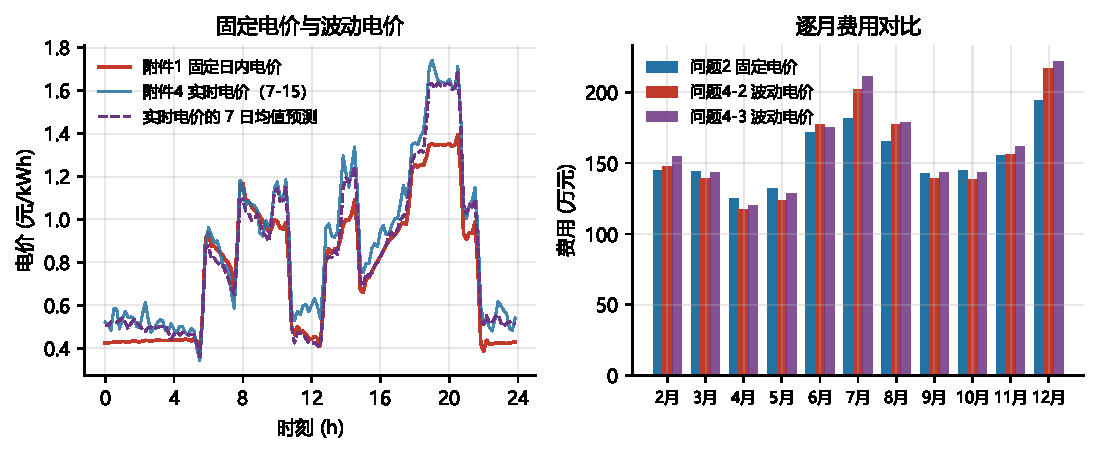
\includegraphics[width=0.95\textwidth]{p4_price.pdf}
  \caption{左：固定电价与实时电价的对比；右：波动电价下各方案逐月费用}
  \label{fig:p4}
\end{figure}

图~\ref{fig:p4} 左图显示实时电价在保持固定日型整体形状的同时叠加了明显的随机波动，7 日均值预测把波动抹平，因此无法捕捉当日的价格尖峰。

\subsection{结果}

\threelinetable{表 10\quad 波动电价与固定电价的结果对比（单位：万元，2025-02-01 至 2025-12-31）}{lrrr}
{项目 & 固定电价 & 波动电价 & 差额}
{对应问题二：计划购电费 & 1570.26 & 1586.77 & $+16.52$ \\
 对应问题二：紧急购电费 & 132.38 & 147.35 & $+14.97$ \\
 对应问题二：\textbf{合计} & \textbf{1702.64} & \textbf{1734.13} & $\mathbf{+31.49}$ \\
 对应问题三：购电费 & 1613.01 & 1622.37 & $+9.36$ \\
 对应问题三：偏差违约费 & 45.43 & 47.07 & $+1.64$ \\
 对应问题三：紧急购电费 & 102.12 & 113.34 & $+11.23$ \\
 对应问题三：\textbf{合计} & \textbf{1760.56} & \textbf{1782.78} & $\mathbf{+22.22}$}

\threelinetable{表 11\quad 问题四指定日期的总费用（元）}{lrr}
{日期 & 问题 4-2 & 问题 4-3}
{2025-03-20 & 46341.46 & 53060.54 \\
 2025-06-21 & 42396.35 & 41099.82 \\
 2025-09-23 & 52841.39 & 53048.42 \\
 2025-12-21 & 75219.74 & 79321.30}

\subsection{价格预测误差的代价}

为了量化价格不确定性本身的成本，本文另外计算了一条\textbf{价格完全信息}的参照线：假设 0:00 就已知当天的全部实际电价，其余设置与问题 4-2 完全相同。该方案全年费用 $17180752.62$ 元，比可实现的方案低
\begin{equation}
17341287.33-17180752.62=160534.71\ \text{元} .
\end{equation}
这就是价格预测误差在问题 4-2 口径下的全部代价，占该方案总费用的 $0.93\%$。这个数字远小于紧急购电所占的比重（$8.5\%$），说明在本数据集上\textbf{电价波动的影响小于负载与光伏预测误差的影响}：实时电价虽然波动幅度不小（标准差 $0.3360$ 元/$\mathrm{kWh}$），但它保留了固定日型的形状，而 7 日均值预测已经抓住了这个形状。

另一个佐证是：问题 4-3 的滚动修正同样有效，紧急购电由 $343800.18$ 降到 $269939.50\,\mathrm{kWh}$，降幅 $7.39$ 万 $\mathrm{kWh}$，与固定电价下的表现一致（$34.38\to26.82$ 万 $\mathrm{kWh}$）。说明滚动修正的价值来自光伏预报的改进，与价格是否波动无关。

\section{模型的检验与灵敏度分析}

\subsection{数值可行性检验}

对四个问题的全部执行方案逐区间回代检验，结果见表 12。能量平衡按
$x_t+PV_t+d_t+E_t=L_t+c_t+w_t$ 核算，储电量与充放电量按式~\eqref{eq:p1soc} 递推。

\threelinetable{表 12\quad 数值可行性检验的最大违反量}{lrrrrr}
{检验项 & 问题二 & 问题三 & 问题 4-2 & 问题 4-3 & 阈值}
{能量平衡残差 / kWh & $4.6\times10^{-13}$ & $2.3\times10^{-13}$ & $2.3\times10^{-13}$ & $2.3\times10^{-13}$ & $10^{-6}$ \\
 储电量越界 / kWh & $0$ & $3.0\times10^{-12}$ & $0$ & $3.6\times10^{-12}$ & $10^{-6}$ \\
 充放电功率越界 / kWh & $0$ & $0$ & $0$ & $1.8\times10^{-12}$ & $10^{-6}$ \\
 售电（负购电量）/ kWh & $0$ & $0$ & $0$ & $0$ & $0$}

另外核对过：五个结果文件的分段值之和与“全天购电量”列完全一致（最大偏差 $10^{-11}$，来自四位小数舍入）；\texttt{result2.xlsx} 的充放电量表共 $2005=1+334\times6$ 行，覆盖 2 月至 12 月全部 334 天，无遗漏。

\subsection{因果性检验}

对问题二至问题四的每一天，程序断言其使用的预测只由第 $d-1$ 天及更早的数据构成；问题三的调整只使用发布时刻不晚于该时刻的预报。以式~\eqref{eq:fc} 与式~\eqref{eq:p3expand} 的实现为例，第 $d$ 天的输入切片上界恒为 $d$（开区间），不存在读取当天未来的可能。

\subsection{参数灵敏度}

以问题二全年总费用 $17026400$ 元为基准，逐项扰动关键参数，结果见表 13。

\threelinetable{表 13\quad 关键参数灵敏度（问题二全年，单位：元）}{llrr}
{参数 & 取值 & 总费用 & 相对基准}
{日前预测窗口 & 前 1 日 & 20866511 & $+3840111$ \\
              & 前 3 日 & 20544768 & $+3518368$ \\
              & \textbf{前 7 日} & \textbf{17026400} & $\mathbf{0}$ \\
              & 前 14 日 & 17150375 & $+123975$ \\
              & 前 30 日 & 17326664 & $+300264$ \\
 安全裕度分位点 & 0.00（不加裕度） & 23959895 & $+6933495$ \\
              & 0.70 & 17163260 & $+136860$ \\
              & \textbf{0.80} & \textbf{17026400} & $\mathbf{0}$ \\
              & 0.90 & 17258273 & $+231873$ \\
 误差样本窗口 & 前 7 日 & 17284369 & $+257969$ \\
              & 前 28 日 & 17026400 & $0$ \\
              & 前 120 日 & 16986934 & $-39467$ \\
 收尾电量约束 & 日循环（本文） & 17026400 & $0$ \\
              & 收尾自由 & 17053078 & $+26678$ \\
 充电效率 $\eta_c$ & 0.85 & 17193129 & $+166728$ \\
              & \textbf{0.90} & \textbf{17026400} & $\mathbf{0}$ \\
              & 1.00 & 16700941 & $-325459$}

三点结论：

\textbf{（1）7 日预测窗口是一个真实的极值点。}窗口从 1 日加长到 7 日，费用从 $2086.7$ 万元迅速降到 $1702.6$ 万元（降幅 $18.4\%$）；再继续加长到 30 日反而回升到 $1732.7$ 万元。原因是短窗口噪声大、误差分位数估不准，长窗口则把季节性的负载水平抹平了。

\textbf{（2）安全裕度分位点对费用极其敏感，且最优值可被理论预测。}不加裕度要多花 $693$ 万元（$40.7\%$），分位点每偏离 $0.1$ 约损失 $13\sim23$ 万元。表 14 进一步验证了式~\eqref{eq:newsvendor}：当紧急购电价改为 $m$ 倍时，理论最优分位点 $q=1-1/m$ 始终优于固定取 $0.8$。

\threelinetable{表 14\quad 紧急购电价比率 $m$ 与最优安全裕度}{crrr}
{$m$ & 理论 $q=1-1/m$ & 按理论 $q$ 的费用 / 元 & 固定 $q=0.8$ 的费用 / 元}
{2.0  & 0.500 & 15604004 & 16232095 \\
 3.0  & 0.667 & 16299627 & 16496864 \\
 5.0  & 0.800 & 17026400 & 17026400 \\
 8.0  & 0.875 & 17648981 & 17820705 \\
 10.0 & 0.900 & 17946676 & 18350242}

\textbf{（3）效率口径与收尾约束的影响是可控的。}充电效率在 $0.85\sim1.00$ 之间变动时，全年费用变化在 $-32.5$ 万到 $+16.7$ 万元之间（不超过 $2\%$），说明“充放电效率 $90\%$”这一歧义的量级有限。收尾约束方面，允许储电量跨日自由漂移反而贵 $2.7$ 万元——因为收尾电量自由时线性规划会把储能一路充到 $10800\,\mathrm{kWh}$ 的上限并长期停在上面（把残值折现的退化行为），所以日循环口径既更贴近题面，也确实更省。

\section{模型的评价与推广}

\subsection{模型优点}

\textbf{（1）用一条恒等式统一了四问的经济逻辑。}式~\eqref{eq:identity} 把执行缺额写成预测误差减去计划弃光量，说明在“严格按计划执行”的口径下，紧急购电只由预测精度和保险水平决定，与储能调度无关。这条恒等式使问题二的“买多少保险”和问题三的“预报值多少钱”变成两个可以独立处理、且都能用闭式公式刻画的子问题。

\textbf{（2）安全裕度有理论最优解而非经验调参。}紧急购电价的 5 倍非对称代价使最优保险量恰好等于预测误差分布的 $0.8$ 分位点。实测全年费用曲线的最低点落在 $q=0.80$，且在 $m=2,3,8,10$ 倍时 $q=1-1/m$ 始终最优，理论预测与数值实验完全吻合，模型的结论不是对某一组数据的过拟合。

\textbf{（3）严格因果且可复现。}问题二至四的每一天都只使用决策时刻之前的信息，全流程由 \texttt{run\_all.py} 一键复现（约 30 秒），所有数值都可由结果文件回读核对。

\subsection{模型缺点}

\textbf{（1）储能严格按计划充放电，牺牲了执行阶段的自适应能力。}这也是式~\eqref{eq:identity} 成立的前提。若允许储能根据实际缺额临时放电，紧急购电可以进一步下降，代价是充放电量偏离计划、SOC 轨迹不再受控。当前口径下电池的应急缓冲作用只能通过“多买”来替代，这是保守的处理。

\textbf{（2）日循环约束放弃了跨日储能。}由于电价日型固定，跨日套利空间本就很小（灵敏度分析显示差值在 $10^{-3}$ 量级），但在连续阴天等场景下放开该约束仍有收益。

\textbf{（3）附件 3 的预报没有被充分利用。}表 7 显示附件 3 的预报误差约为历史均值的 $2.4$ 倍，若把两路信息按历史表现加权融合，预测误差还能进一步下降。本文为了严格对应题面给定的信息结构，没有做这一步。

\subsection{推广方向}

本文的“预测误差 + 报童裕度 + 滚动修正”框架不限于微网购电。凡是满足以下三条的场景都可以直接套用：存在一个按计划结算的基础量、偏差按非对称价格事后结算、并且有可逐步更新的预测。典型的例子包括工业用户的需量申报与偏差考核、电力市场的日前申报与实时平衡、以及供热的以热定电与调峰补偿。模型中唯一需要替换的部分是预测模块——把 7 日历史均值替换为该场景的专用预测即可，安全裕度的分位点仍由 $q=1-1/m$ 给出，其中 $m$ 是偏差惩罚倍数。


\newpage
\referencescn
\newpage
\appendixcn

\end{document}
